\section{Implementation}
In order to gain deeper insights into the operational dynamics and performance characteristics of
decentralized social media platforms, our team has undertaken an innovative demonstration project
leveraging the capabilities of Arroyo, a cutting-edge stream processing framework, to develop and
implement a sophisticated event processing system specifically designed to monitor and analyze
real-time activities across the Mastodon social network federation. This comprehensive monitoring
solution serves multiple strategic objectives, including the evaluation of user engagement patterns,
the assessment of network performance metrics, and the development of a more nuanced understanding
of how decentralized social media architectures function in practice. Through this implementation,
we aim to not only demonstrate the practical applications of stream processing technology in social
media analytics but also to contribute valuable insights to the growing body of knowledge
surrounding alternative social networking models that prioritize user privacy, data sovereignty, and
community-driven governance structures.

\subsection{Mastodon}
Mastodon represents a new approach to social networking through decentralized architecture. Rather
than operating as a single centralized platform controlled by one company, Mastodon functions as a
network of independently operated servers, known as instances. Each instance runs on open-source
software and communicates with other instances through a standardized protocol called ActivityPub
\cite{La_Cava_2021,w3c_2018}.

Mastodon has emerged as the most prominent platform within the Fediverse, offering functionality
comparable to traditional social media services. Users can share short-form content called "toots"
(similar to tweets) and amplify others' content through "boosts" (similar to retweets). The platform
also incorporates community-focused features reminiscent of Reddit, with independent communities
managed through separate instances, each with its own moderation policies.

The federated architecture of Mastodon serves as the foundation for our demonstration results,
utilizing a sophisticated event-driven approach to track and analyze instance activity across the
network. From a technical implementation perspective, the system operates by monitoring update
events across all participating Mastodon instances through a specialized Server-sent event
protocol \cite{html_standard_2024}, which broadcasts these events to a designated endpoint whenever a
user performs any update action within the network \cite{mastodon_ggmbh_2022}. Our technical
infrastructure systematically processes this event stream by first consuming the incoming events,
then performing data extraction to isolate the instance domain information from the event payload,
followed by implementing a rolling time-window aggregation mechanism that operates on 5-minute
intervals to calculate the frequency of updates originating from each domain instance. The
culmination of this processing pipeline results in the identification and selection of the five most
active instances, determined by their respective update frequencies, which provides valuable
insights into the distribution of user activity across the Mastodon federation network and helps us
understand the patterns of engagement within the decentralized social media landscape.

\subsection{Set Up Infrastructure}
For our experimental infrastructure implementation, we made a strategic decision to deploy Arroyo on
a Raspberry Pi model 3B+, a choice that aligns with our objectives to evaluate stream processing
capabilities on accessible hardware platforms. Our server configuration encompasses a 1.4GHz 64-bit
quad-core ARM Cortex-A53 processor complemented by 1 GB LPDDR2 SDRAM, with network connectivity
provided through Gigabit Ethernet, establishing a robust foundation for our testing environment.
This deliberate selection of commodity hardware serves multiple research purposes, primarily
enabling us to conduct detailed performance monitoring of Arroyo while simultaneously investigating
its operational characteristics on consumer-grade equipment. The decision holds particular relevance
given the industry's current trajectory toward increased utilization of edge computing devices in
stream processing applications. Our implementation offers an interesting comparative analysis
opportunity against established solutions like Apache Flink, which operates within the Java Virtual
Machine (JVM) ecosystem; in contrast, Arroyo's implementation in Rust suggests potentially lower
resource overhead, making it an intriguing candidate for resource-constrained environments. This
architectural choice not only supports our immediate research objectives but also provides valuable
insights into the feasibility of deploying modern stream processing solutions on accessible hardware
platforms, contributing to the broader discussion of edge computing capabilities in data processing
applications.

For this project, we decided to use a Raspberry Pi model 3B+ to host the Arroyo, a choice that
aligns with our objectives to evaluate stream processing capabilities on accessible hardware
platforms. Some machine specifications for our server includes: a 1.4GHz 64-bit quad-core ARM
Cortex-A53 processor, a 1 GB LPDDR2 SDRAM, internet connection through Gigabit Ethernet
\cite{raspberrypi}. This deliberate selection of commodity hardware serves multiple research
purposes, primarily enabling us to conduct detailed performance monitoring of Arroyo while
simultaneously investigating its operational characteristics on consumer-grade equipment. The
decision holds particular relevance given the industry's current trajectory toward increased
utilization of edge computing devices in stream processing applications. In contrast with Apache
Flink, which was written in Java and execute on Java Virtual Machine (JVM), Arroyo's
implementation in Rust suggests potentially lower resource overhead, making it an intriguing
candidate for resource-constrained environments. This architectural choice not only supports our
immediate research objectives but also provides valuable insights into the feasibility of deploying
modern stream processing solutions on accessible hardware platforms, contributing to the broader
discussion of edge computing capabilities in data processing applications.

\begin{figure}[H]
    \centering
    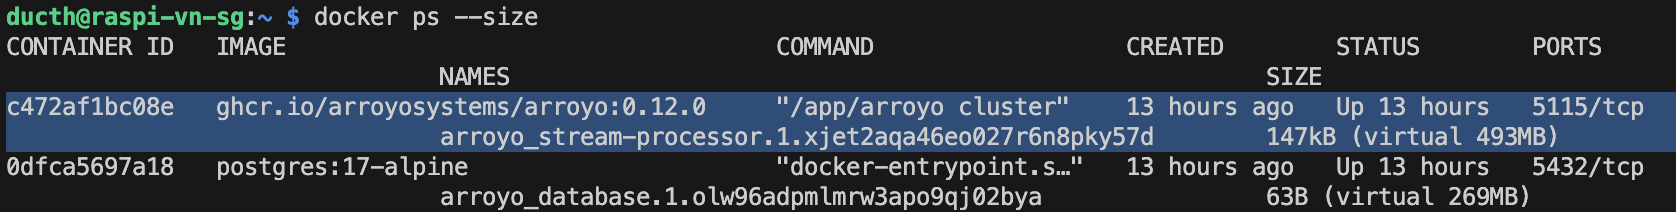
\includegraphics[width=\textwidth]{Images/docker_stack_deployment.png}
    \vspace{1em}
    \caption{Displaying deployment in Docker}
    \label{fig:docker_stack}
\end{figure}

In alignment with contemporary best practices in containerization and microservices architecture,
our deployment infrastructure leverages Docker Stack \cite{docker_stack} technology to orchestrate
and manage the operational components of our system, specifically focusing on two primary services:
the Arroyo server implementation and its associated PostgreSQL database instance. This containerized
approach not only ensures consistent deployment across different environments but also facilitates
sophisticated resource management and monitoring capabilities. Our performance analysis, as
illustrated in the accompanying system metrics visualization \ref{fig:docker_stack}, demonstrates
remarkably efficient resource utilization patterns, with both the Arroyo server and PostgreSQL
database maintaining notably conservative memory footprints that aggregate to approximately 800 MB
of total system memory consumption. This impressive resource efficiency validates our architectural
decisions and suggests substantial potential for scaling our implementation across various
deployment scenarios, from development environments to production systems, while maintaining optimal
performance characteristics and resource utilization patterns.

Our team source code for the \texttt{docker-compose.yaml} can be reviewed on our GitHub repository.

\subsection{Arroyo Console guide}
After successfully setting up and deploying Arroyo on our server infrastructure, we moved forward
with designing and implementing the monitoring pipeline that would help us achieve our project
objectives. Arroyo comes equipped with a user-friendly interface that makes the process of
developing and deploying data processing jobs surprisingly straightforward and intuitive. To begin
creating our monitoring solution, we simply navigated to the Arroyo Console, which serves as the
central hub for managing all pipeline-related operations. The interface presents a clean and
straightforward layout where users can find the \textbf{Create Pipeline} button prominently
displayed, marking the starting point for building new data processing workflows. This streamlined
approach to pipeline creation reflects Arroyo's overall design philosophy of making stream
processing more accessible while maintaining the powerful capabilities needed for complex data
analysis tasks. The simplicity of the interface proved to be a significant advantage for our team,
allowing us to focus more on the actual implementation of our monitoring logic rather than getting
caught up in complicated setup procedures or configuration details.

\begin{figure}[H]
    \centering
    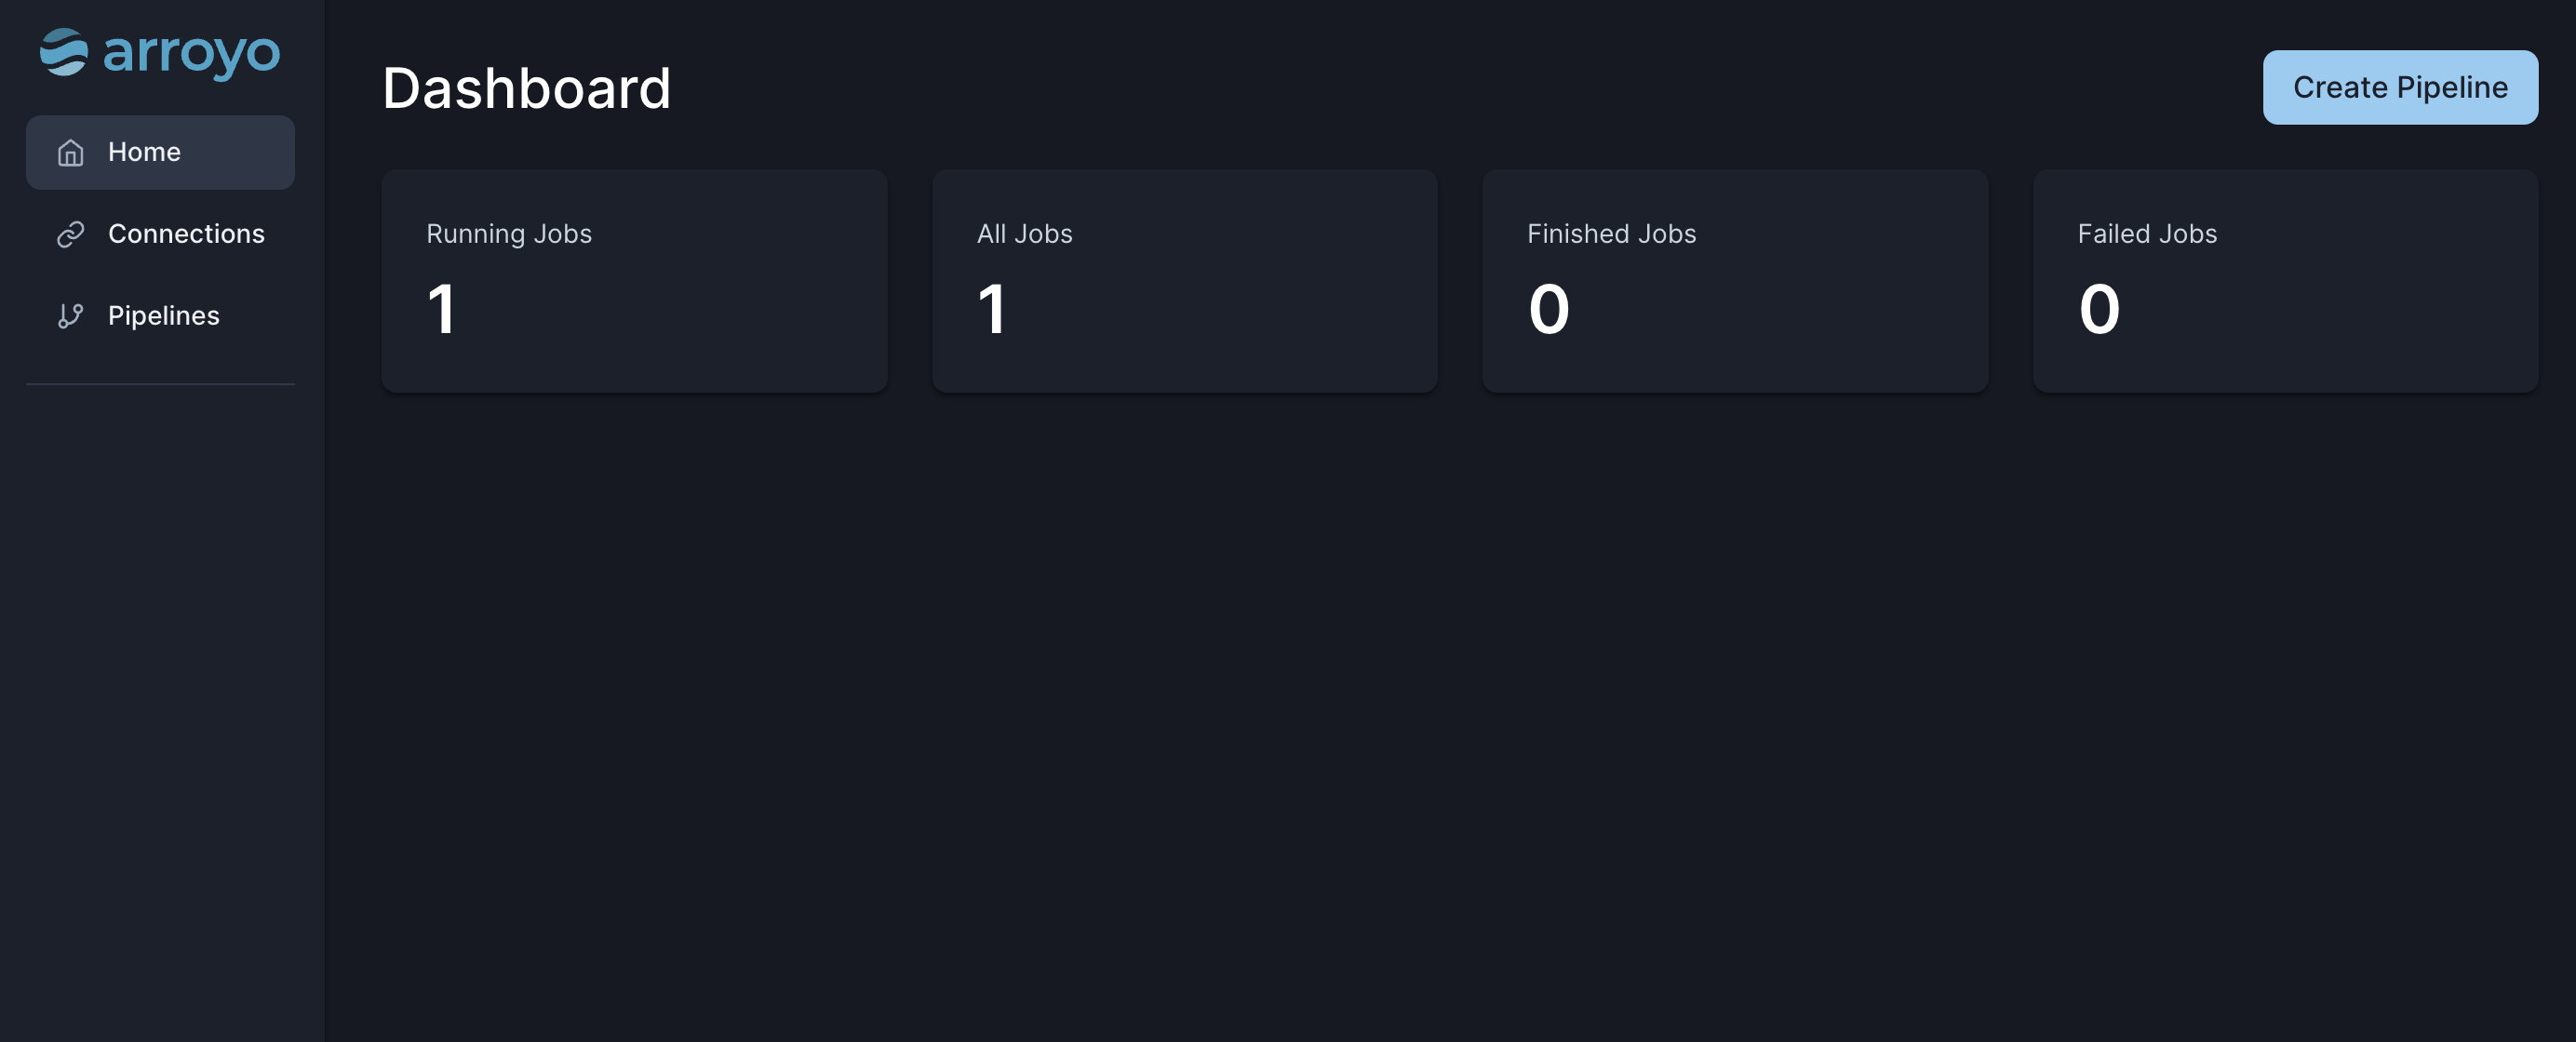
\includegraphics[width=\textwidth]{Images/arroyo_dashboard.png}
    \vspace{1em}
    \caption{Arroyo dashboard with our demo job running}
    \label{fig:arroyo_dashboard}
\end{figure}

Arroyo offers a straightforward and user-friendly Interactive Development Environment (IDE),
designed to simplify the process of working with data. Within this IDE, users can effortlessly write
SQL queries to read and manipulate data, enabling efficient calculations and transformations. The
\textbf{Preview} feature, accessible via the menubar, allows users to quickly preview the output of
their queries, providing immediate feedback and facilitating a more streamlined development cycle.
This rapid feedback loop helps users fine-tune their queries before proceeding to deployment. Once
the query meets the desired specifications, the \textbf{Launch} action can be used to deploy the
code for actual execution, making the transition from development to production both seamless and
efficient.

\begin{figure}[H]
    \centering
    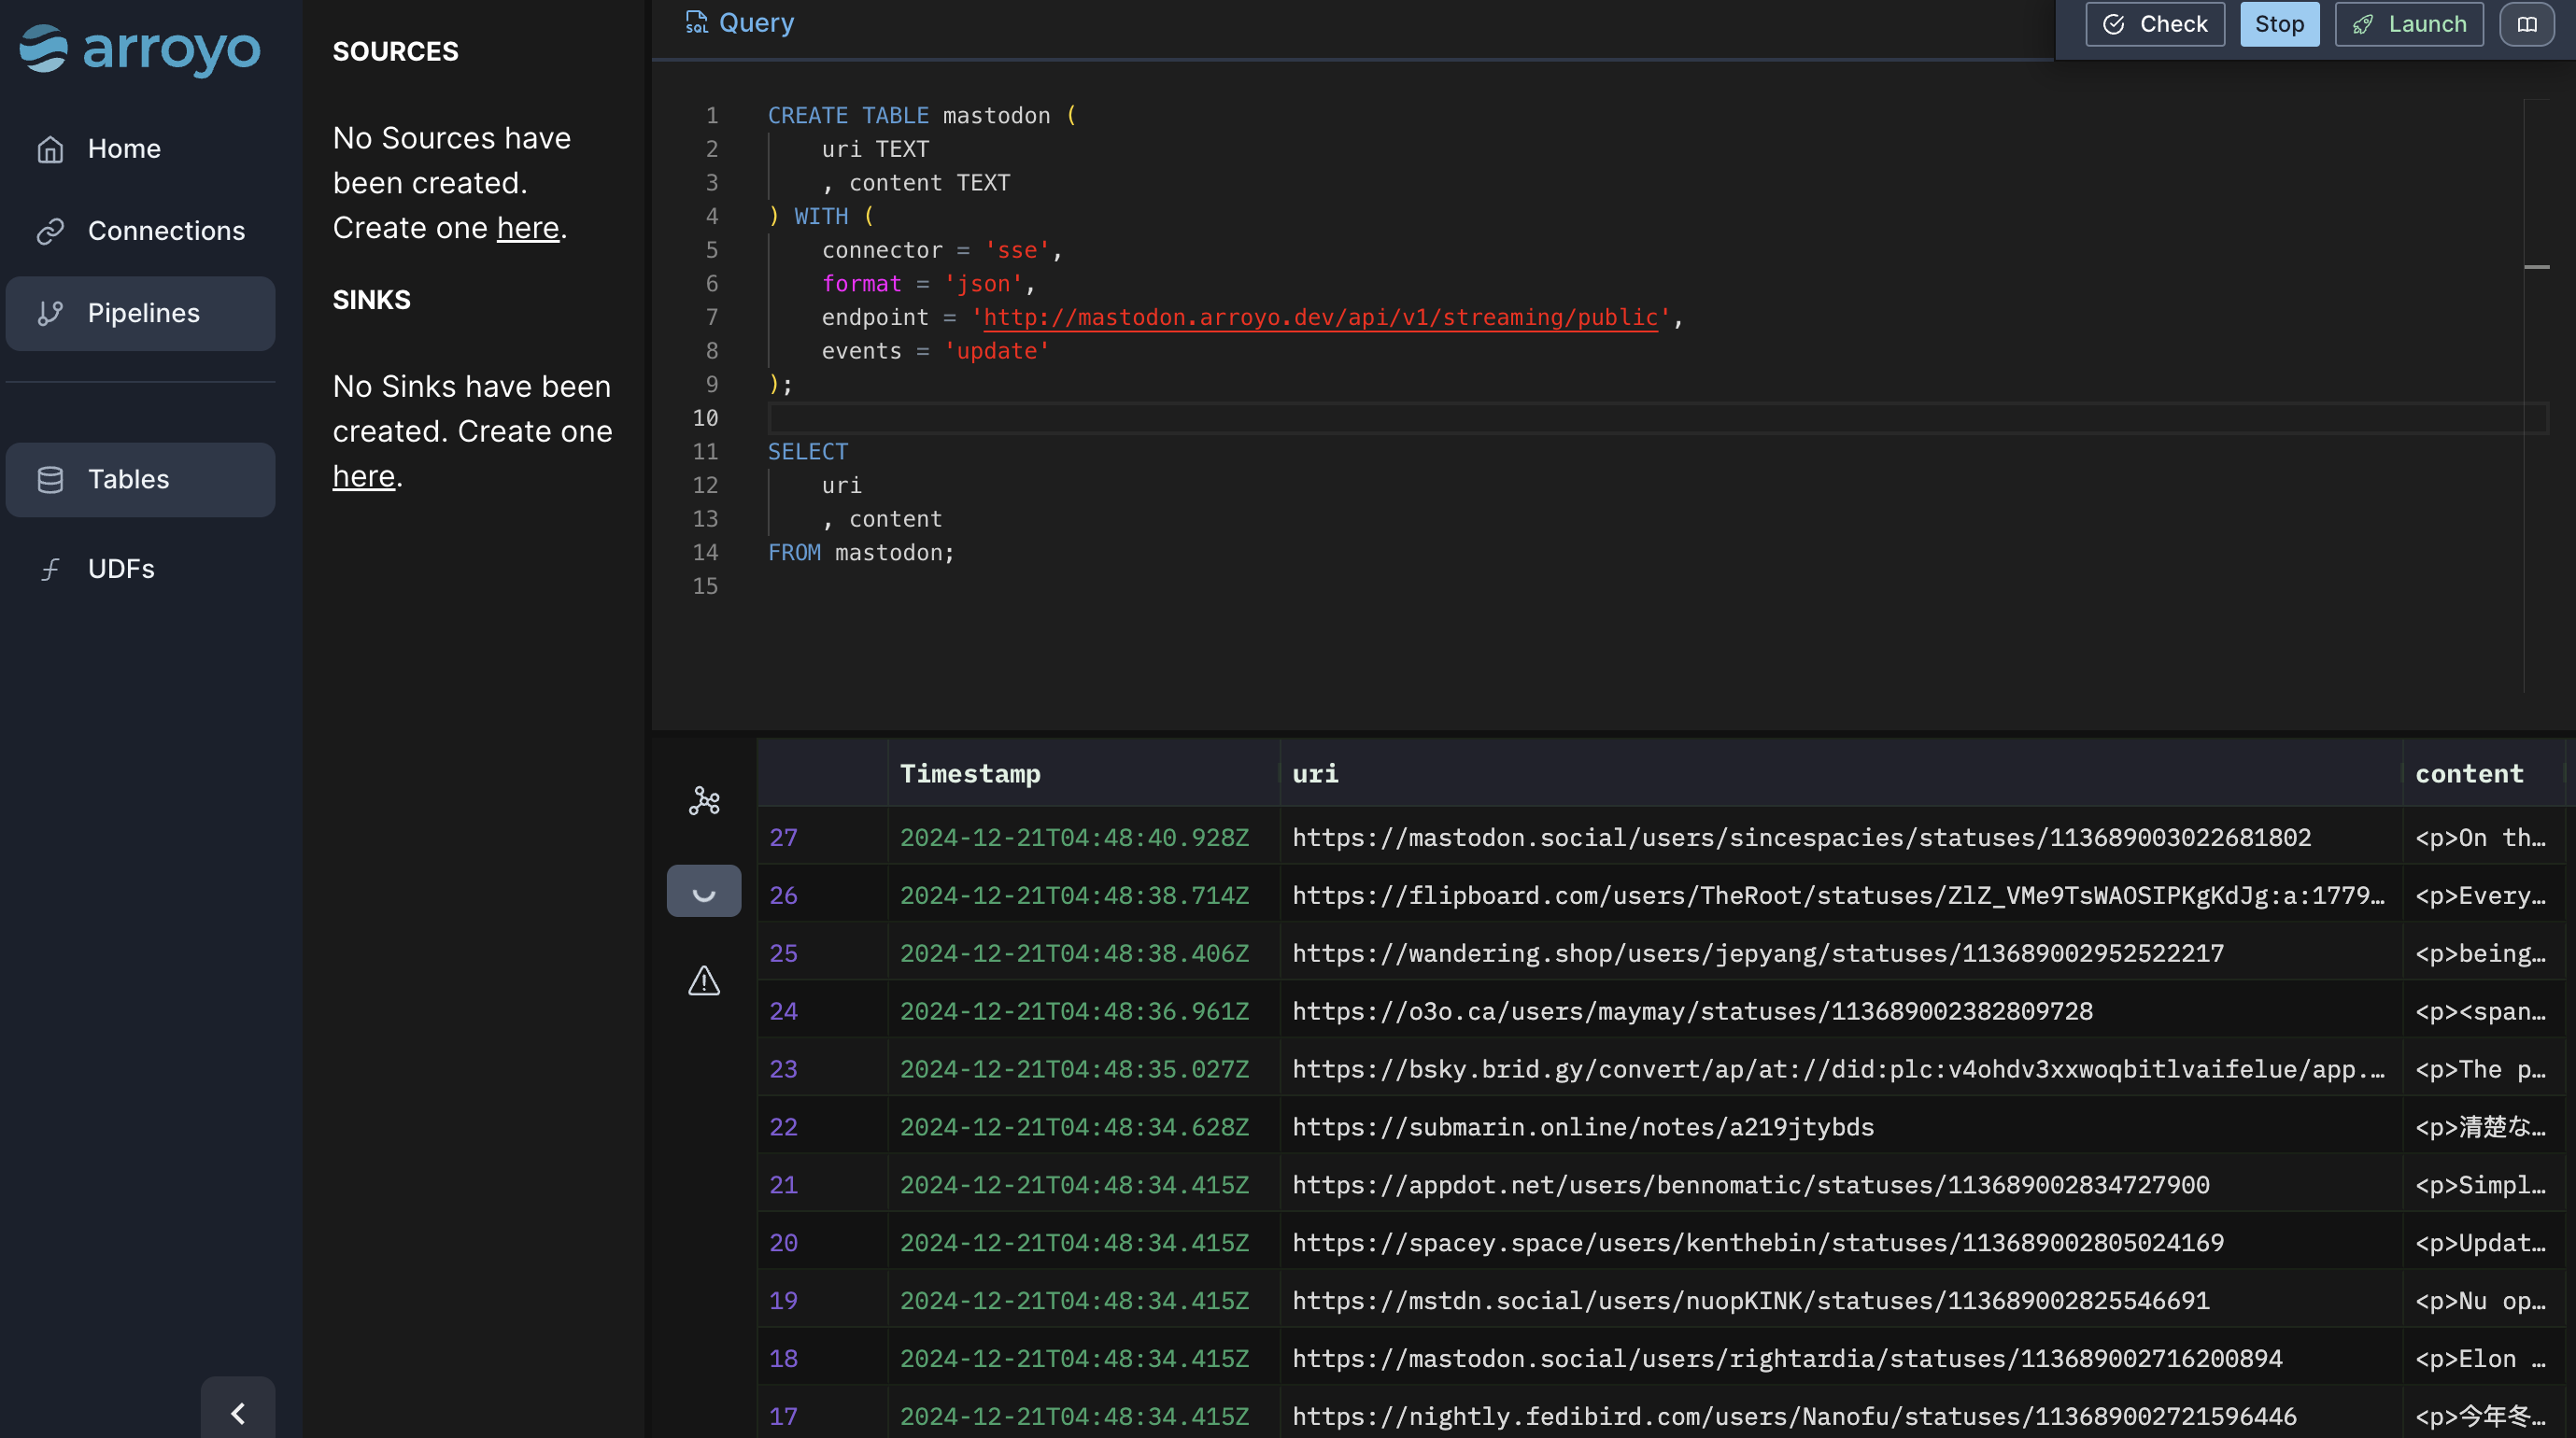
\includegraphics[width=\textwidth]{Images/arroyo_ide.png}
    \vspace{1em}
    \caption{Arroyo IDE}
    \label{fig:arroyo_ide}
\end{figure}

Arroyo also provides a highly intuitive dashboard that offers comprehensive monitoring capabilities
for running job details. This dashboard is equipped with a range of features designed to enhance
usability and insight: it visually represents the query tree or query plan of the task, enabling a
clear understanding of the job's structure; it allows users to tail the outputs of the job,
providing real-time visibility into its operation; and it offers detailed technical insights into
checkpoints, such as memory usage for each operator, the duration between operator lags, and other
performance metrics. These features collectively support a deeper understanding of the job's
behavior during deployment, making it easier for operators to quickly identify and address any
abnormalities or inefficiencies that may arise during execution.

\begin{figure}[H]
    \centering
    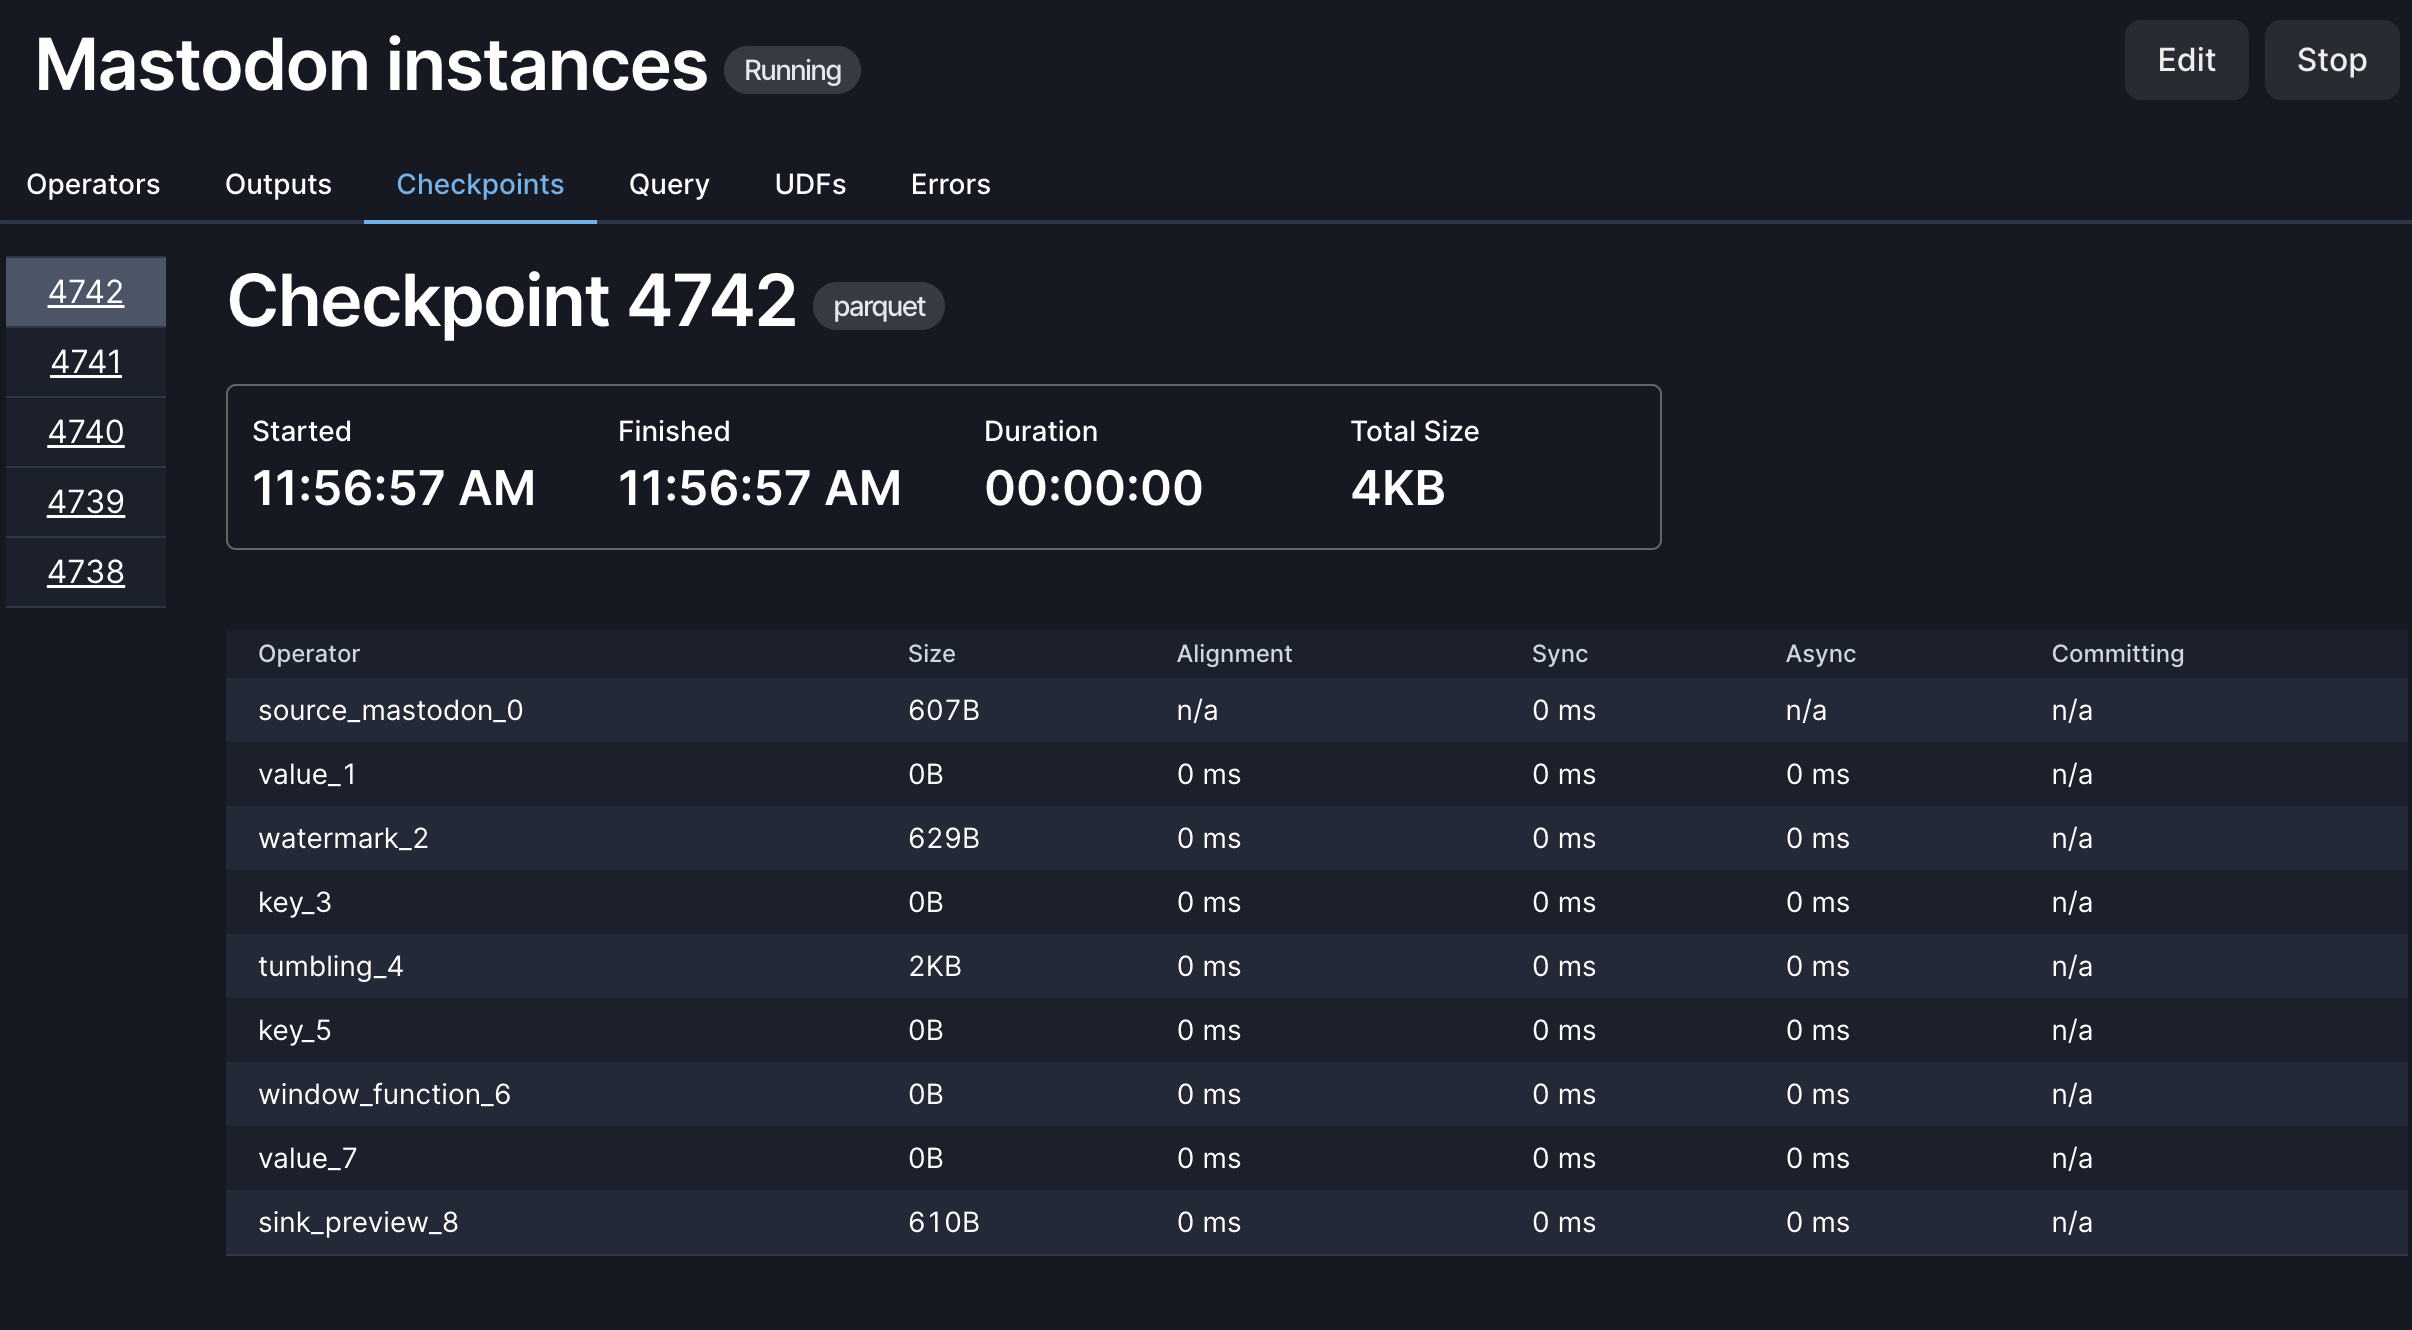
\includegraphics[width=\textwidth]{Images/arroyo_job_checkpoints.png}
    \vspace{1em}
    \caption{Details about a checkpoint of our demo job}
    \label{fig:arroyo_job_checkpoints}
\end{figure}

\subsection{Develop Instances Count Measurement}
We now describe in depth the code to accomplish the aforementioned objective.

\begin{lstlisting}[language=SQL]

CREATE TABLE mastodon (
    uri TEXT
) WITH (
    connector = 'sse',
    format = 'json',
    endpoint = 'http://mastodon.arroyo.dev/api/v1/streaming/public',
    events = 'update'
);

\end{lstlisting}

First, this snippet of code will create a \textbf{Source} for incoming data into the system. Here,
by using table as an abstraction, Arroyo simplifies the process of reading or writing to any other
system. Any type of messaging fabrics: Apache Kafka, MQTT or SSE can be represented in a relational
model. According to Mastodon documentation, incoming events are JSON-encoding, with a sample
structure similar to below. As you can see, the schema of the object has a high complexity.

\begin{lstlisting}[language=Python]
{
  "id": "108914327388663283",
  "created_at": "2022-08-30T23:05:46.839Z",
  "language": null,
  "uri": "https://letsalllovela.in/objects/e9cebb0c-7c75-414f-9608-20b5628e52d7",
  "content": "<span class=\"h-card\"><a class=\"u-url mention\" href=\"https://pl.nulled.red/users/disarray\" rel=\"nofollow noopener noreferrer\" target=\"_blank\">@<span>disarray</span></a></span> glad i was able to help",
  "account": {
    "id": "464472",
    "username": "freon",
    "acct": "freon@letsalllovela.in",
    "created_at": "2018-08-18T00:00:00.000Z",
    "emojis": [],
    "fields": [
      { "name": "pronouns", "value": "emacs/xemacs (or he/they)", "verified_at": null },
      { "name": "age", "value": "23.66667", "verified_at": null }
    ]
  },
  "media_attachments": [],
  "mentions": [
    { "id": "107946650784398271", "username": "disarray", "url": "https://pl.nulled.red/users/disarray", "acct": "disarray@pl.nulled.red" }
  ],
}
\end{lstlisting}

However, to achieve our result, we will focus primarily in the field \texttt{uri}. Because of this,
Arroyo helps us extract and parse this field into a separate column by setting the format to
\texttt{'json'}. That way, we can skip the step of actual parsing the JSON and get the property
(using Arroyo \texttt{json\_get} method).

\begin{lstlisting}[language=SQL]
WITH extract_domain AS (
    SELECT
        split_part(
            substr(uri, strpos(uri, '://') + 3),
            '/',
            1
        ) AS instance_domain
    FROM mastodon
)
\end{lstlisting}

Arroyo also supports the syntax of Common Table Expression (or CTE). This will support us with
enhancing code readability, by replacing nested \texttt{SELECT} statement with table representing
each step of the final transformation. For the first transformation, our team extracted the domain
name section from the URI, which should reside between a scheme (such as \texttt{https://}) and a
forward slash \texttt{/}. Arroyo SQL also supports many built-in string manipulation methods, like
\texttt{strpos} to find a position of a substring within a text, \texttt{substr} to extract a
substring between a beginning and ending position, and \texttt{split\_part} to split a string into
multiple substring based on a delimiter, and select a result of the splits.

\begin{lstlisting}[language=SQL]
, instance_domain_count AS (
    SELECT
        TUMBLE(interval '5 minutes') AS window
        , instance_domain
        , COUNT(*) AS cnt
    FROM extract_domain
    GROUP BY window, instance_domain
)
, instance_domain_sort AS (
    SELECT
        window
        , instance_domain
        , cnt
        , ROW_NUMBER() OVER (PARTITION BY window ORDER BY cnt DESC) AS order
    FROM instance_domain_count
)
SELECT
    window
    , instance_domain
    , cnt
FROM instance_domain_sort
WHERE order <= 5;
\end{lstlisting}

The next two steps is for our team to perform the complex aggregation on the incoming stream. To
achieve our object, we performed aggregation on data based on fixed-size, non-overlapping windows of
event incoming interval (which is also called \textbf{Tumbling Windows}). Then, we count for the
number of updates for each group of the instances. Finally, \texttt{ROW\_NUMBER()} is used to rank
the instance based on their event counts, partition per interval window. The final \texttt{SELECT}
then write out the result, but as we only interest in the top 5 mostly active instances, the
\texttt{WHERE} clause does the filtering step.

\begin{figure}[H]
    \centering
    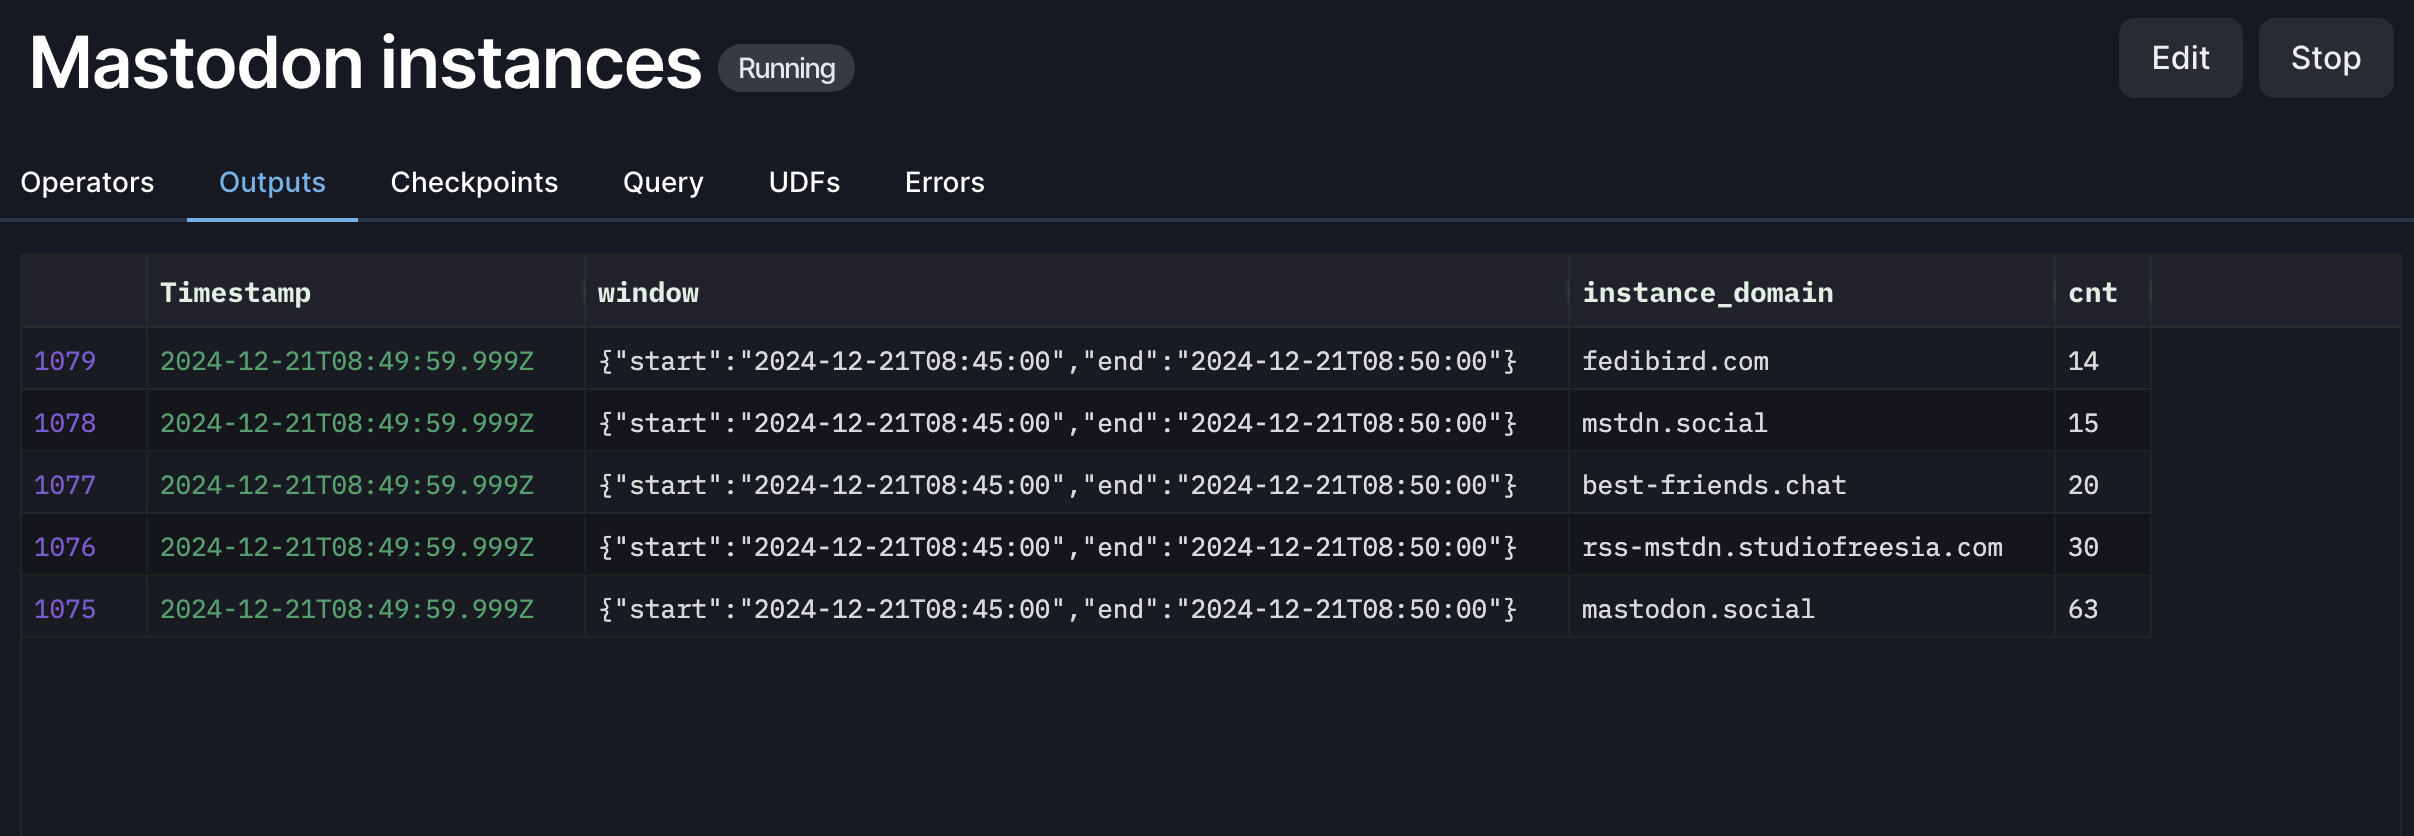
\includegraphics[width=\textwidth]{Images/mastodon_instance_count.png}
    \vspace{1em}
    \caption{Top 5 Mastodon instances within our sampling interval}
    \label{fig:mastodon_instance_count}
\end{figure}

The outcome is a table with a schema in figure \ref{fig:mastodon_instance_count}. Here, it includes
a window of processing interval, the domain name of the instance and its corresponding count. Most
of the time, \hyperref{https://mastodon.social/}{mastodon.social} will be the most active instance.
It was not a surprise when considering that this instance has a high popularity, and to most people
can be considered as the default server for Mastodon.